\documentclass{article}
\usepackage[utf8]{inputenc}
\usepackage{amsmath,amsfonts,amssymb}
\usepackage{graphicx}
\usepackage{booktabs}

\usepackage{lipsum}

\newtheorem{theorem}{Model}[section]
\newtheorem{corollary}{Corollary}[theorem]
\newtheorem{proof}{Proof}[corollary]

\title{Lab Report 1: Analysis on Period vs. Angle and Q Factor of Pendulum}
\author{Zixuan Fan}
\date{09/18/2023}

\begin{document}

\maketitle
\section{Introduction}

In this lab report, I will analyse how the period (T) of my pendulum depends on the angle ($\theta$), as well as measure the Q (quality) factor of said pendulum. The damped harmonic oscillator model will provide a method for us to calculate the Q Factor.

\section{Experimental Set-up}

My experimental set-up for the pendulum will be composed of a golf ball hang from a horizontal wooden stand with double wool strings, as demonstrated in \textbf{Figure 1}:

\begin{figure}[!htb]
	\centering
	\includegraphics[scale=0.05, angle = 270]{experimental_setup_pendulum.jpg}
	\caption{Experimental Set-up of The Pendulum}
	\label{fig_angle}
\end{figure}

\noindent The pendulum will have a vertical length of 37.5 $\pm$ 0.1cm, and it will be released from angle 1.57 $\pm$ 0.01 rad

\subsection{Justification for Experimental Set-ups that Reduce Errors}

The reason I hang the pendulum with two strings, instead of sing the traditional single-string pendulum, is to make sure the pendulum swings in the same plane throughout its motion. Had a single-string pendulum been used, the pendulum would likely swing in circles.\\

\noindent I also carved two grooves at the point where the string sits. This makes sure that the string doesn't slip on the surface of the wooden stand during the pendulum's motion. These two design decisions eliminate potential systematic errors.

\subsection{Justification for Experimental Set-ups that Maintain Symmetry}

In order to maintain symmetry on both sides of the pendulum, I specifically released and recorded the pendulum from both the negative(left) side and the positive(right) side. Recording data from both sides reduces errors in regard of asymmetry, as the experimental set-up will certainly be asymmetrical simply due to nature not being perfect.\\

\noindent Even though the asymmetry in my set-up is unavoidable, I can still reduce this asymmetry by making the resting position of the pendulum as close to the center line as possible. I attempted to achieve this by sliding the knot on the string to the lowest point on the wooden stand, which ensures the direction of the string is normal to the surface of the wooden stand, thereby overlapping with the imaginary center line.

\section{Data Analysis}

Through releasing the pendulum at 90 degree from both side of the wooden stand, and recording the period(the time it takes to complete one back-and-forth swing) at certain angles(15 degree less than the previous angle, until it reaches 30 degree) inside the tracker application, we were able to gather a table of data on the period and their corresponding release angle for the pendulum, as demonstrated in \textbf{Table 1}: \\

\begin{center}(Note that a positive angle implies the release angle to the right side, and a negative angle implies the release angle to the left side)
\end{center}

\begin{table}[!htb]
\caption{Period of Pendulum and Their Corresponding Angle}
\label{table_angle}
\begin{center}
\begin{tabular}{*5c}
\toprule
	Angle(rad) & \multicolumn{4}{c}{Period(s)}\\
\midrule
	{} & Trial 1 & Trial 2 & Trial 3 & Average\\
	1.57 ($\frac{\pi}{2}$) & 1.32 & 1.27 & 1.29 & 1.29\\
	-1.57 (-$\frac{\pi}{2}$) & 1.32 & 1.30 & 1.30 & 1.31\\
	1.31 ($\frac{5\pi}{12}$) & 1.22 & 1.22 & 1.22 & 1.22\\
	-1.31 (-$\frac{5\pi}{12}$) & 1.25 & 1.23 & 1.23 & 1.24\\
	1.05 ($\frac{\pi}{3}$) & 1,17 & 1.22 & 1.17 & 1.184\\
	-1.05 (-$\frac{\pi}{3}$) & 1.18 & 1.17 & 1.22 & 1.189\\
	0.79 ($\frac{\pi}{4}$) & 1.17 & 1.15 & 1.17 & 1.16\\
	-0.79 (-$\frac{\pi}{4}$)& 1.15 & 1.13 & 1.13 & 1.14\\ 
	0.52 ($\frac{\pi}{6}$) & 1.167 & 1.133 & 1.117 & 1.14\\ 
	-0.52 (-$\frac{\pi}{6}$) & 1.12 & 1.10 & 1.12 & 1.11\\
\midrule
	\multicolumn{5}{c}{Uncertainties}\\
\midrule
	$\pm$0.01 & $\pm$0.001 & $\pm$0.01 & $\pm$0.01 & $\pm$0.01 \\
\bottomrule
\end{tabular}
\end{center}
\end{table}

\subsection{Justification for Measurements of Uncertainty}
The measurements for angles are done using an angle-meter with a step of $\pm$1 degree, equivalent to $\pm 1*\pi/180= \pm0.02$ in rad, as observable in \textbf{Figure 1}. Since the angle-meter is an analogue instrument, the uncertainty of Angle should be $\pm 0.02/2= \pm0.01$ rad.\\

\noindent The measurements for periods are done using a digital tracker with a step of 0.01 second. Since the tracker is a digital instrument, the uncertainty of period should be $\pm$ 0.01 second.

\subsection{Importing Data into graphs}

\subsubsection{Graphing and Analysing Figure 2}

Importing the data in \textbf{Table 1} into a provided program, we were able to graph the relationship between the period of pendulum and their corresponding release angles in \textbf{Figure 2}:\\

\begin{figure}[!htb]
	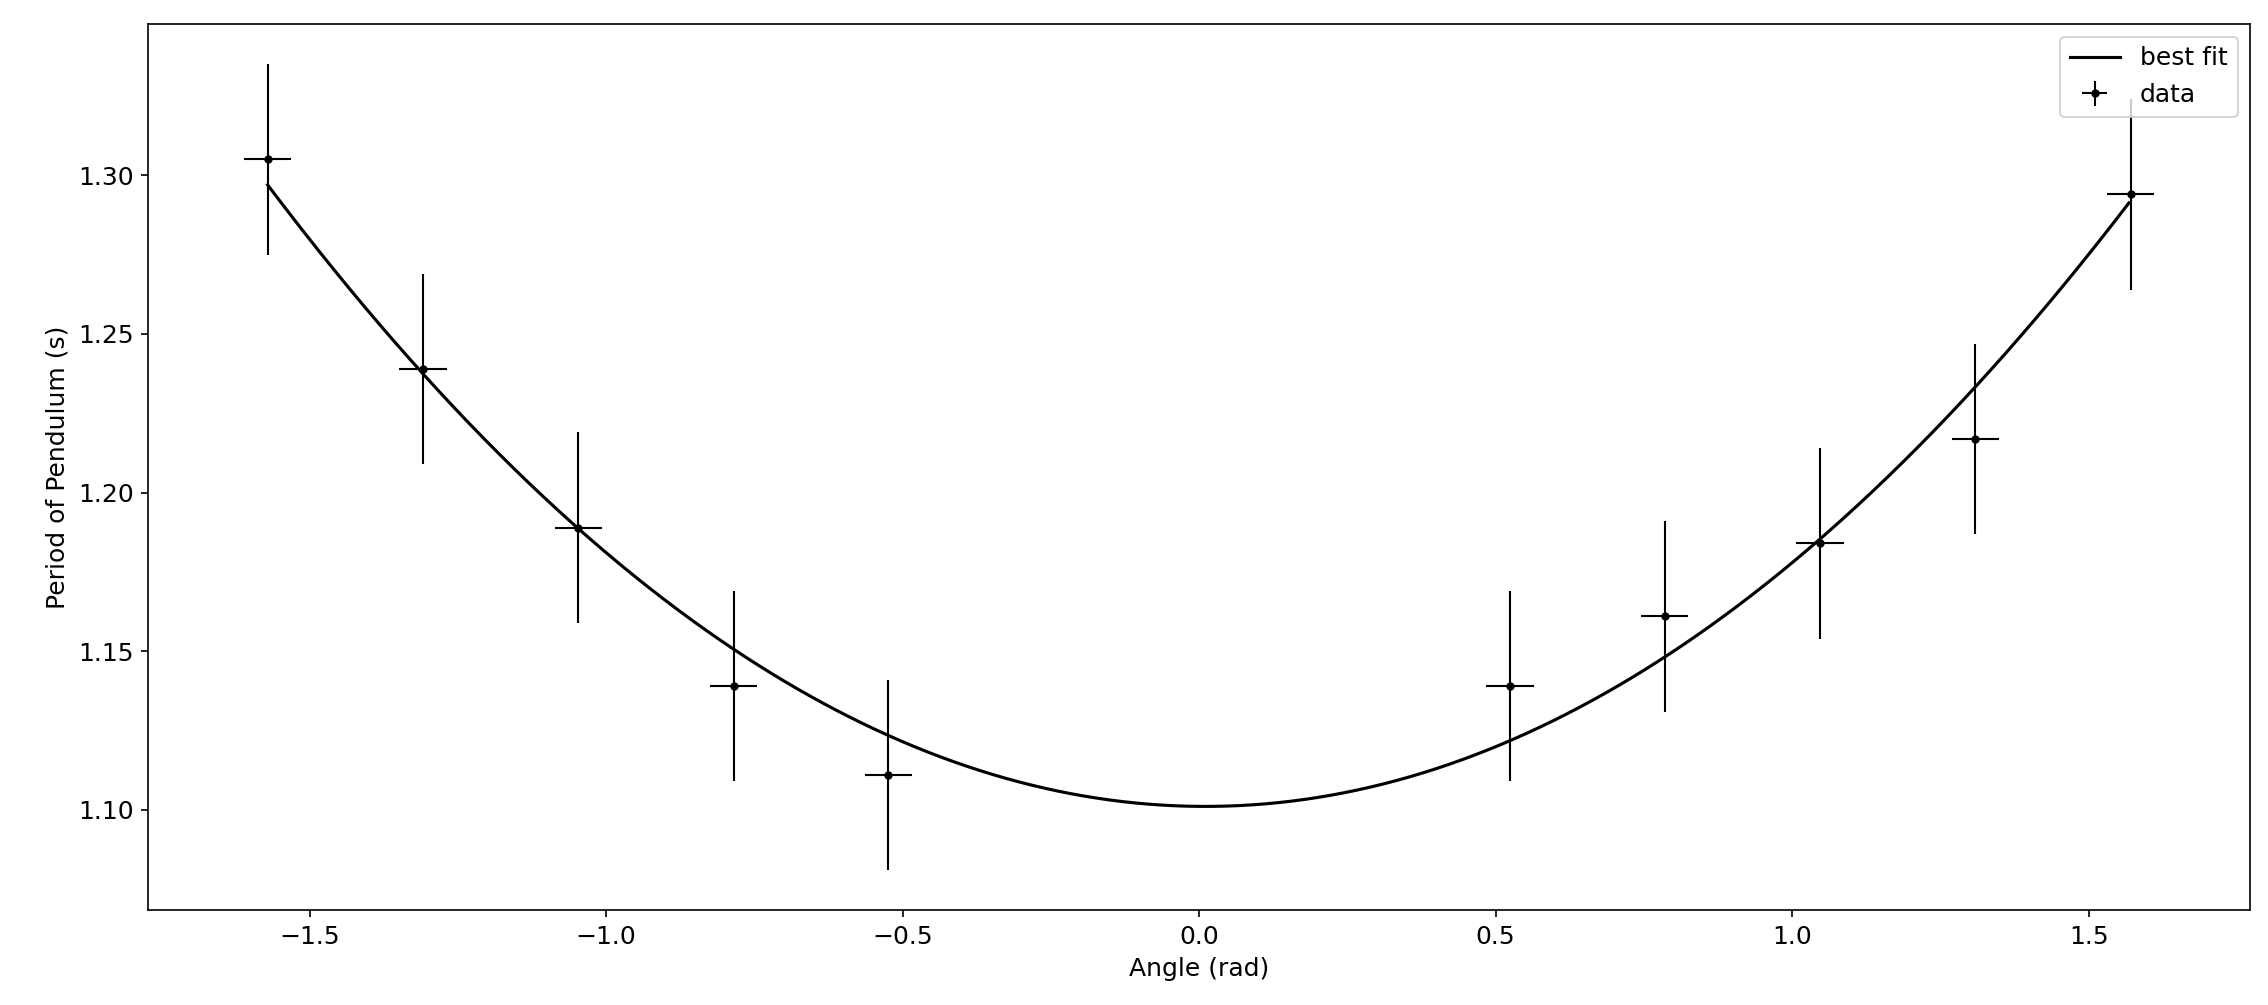
\includegraphics[scale=0.4]{fig_angle.png}
	\caption{Period of Pendulum (s) vs. Angle (rad)}
	\label{fig_angle}
\end{figure}

\noindent Note that the horizontal error bar has a length of $\pm$ 0.01 rad, and the vertical error bar has a length of $\pm$ 0.01 second. \\

\noindent It is observable from \textbf{Figure 2}, that the period decreases exponentially as the angle gets closer to 0 rad. \\

\noindent However, this decrease only happens over an interval of approximately 0.20, which is a minuscule and ignorable decrease, as there are multiple factors of error that could've caused this decrease, which will be discussed in the next subsection.

\subsubsection{Errors Present in Graphing Figure 2}

It is worth noting that there are two systematic error factors which could have caused the decrease, one being the lesser friction experienced between the string and the wooden stand when the pendulum swings at smaller angles, and the other one being the lesser air-resistance experienced when the pendulum swings at smaller angles.


\subsubsection{Graphing and Analysing Figure 3}

Upon tracking the decay of pendulum's amplitude starting from 75  $\pm$ 0.5 degree, or 1.31 $\pm$ 0.01 radian, I am able to plot a graph between the angle of pendulum with respect to time , as demonstrated in \textbf{Figure 3}:\\

\begin{figure}[!htb]
	\centering
	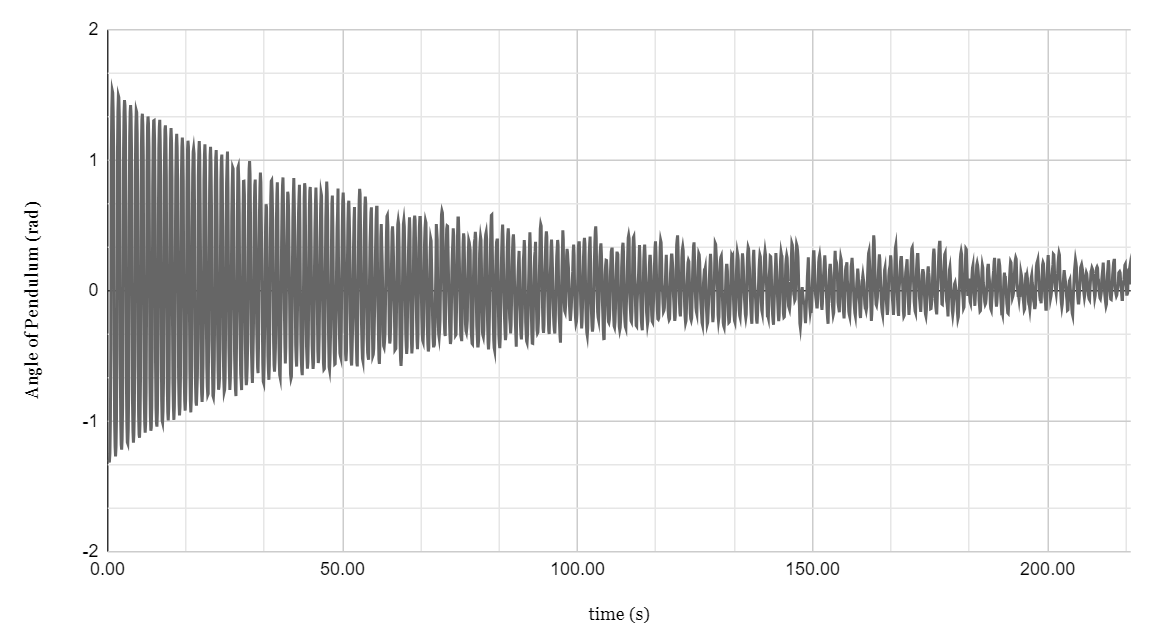
\includegraphics[scale=0.53]{Pendulum_Decay_Chart1.png}
	\caption{Angle of Pendulum (Rad) vs. Time (s)}
	\label{fig_angle}
\end{figure}

\noindent It is observable from \textbf{Figure 3} that the maximum amplitude of the pendulum decreases exponentially as time increases.
\subsubsection{Errors Present in Graphing Figure 3}

To determine the precise location and it's respective angle, I used a digital application named tracker to track the center of mass of the golf ball. However, an error may arise from this practice, in that the location I chose for the center of mass of the golf ball may not be accurate to it's real location. \\

\noindent This is attributable to both human errors, as well as the fact that the ball has a non-zero impulse during certain frames, which can also affect my measurement for the precise location of the center of mass.\\

\noindent This factor of error is random error. It will increase the random fluctuation of the data and thereby making my graph appear less smoother.

\subsection{Q Factor Calculation}
\subsubsection{Determine Q Factor through Estimating Period}

Using the provided mathematical model of the damping angle of the pendulum, as shown in \textbf{Model 3.1}:

\begin{theorem}[Model of Damped Harmonic Motion] ~ %%%

 \[\theta(t) = \theta_0 e^{-t/\tau} \cos(2\pi \frac{t}{T}+\phi_0)\] \label{model_1}
The predicted period would be: \[T\simeq2\sqrt{L}\] \label{model_2}
As engineers, instead of using $\tau$, the Q Factor is more commonly seen, defined as: \[Q=\pi\frac{\tau}{T}\] \label{model_3}

\end{theorem}

\noindent I will be able to derive the Q Factor for my pendulum:\\

Arbitrarily choosing $t = 50.03$,

\[\therefore \theta(50.03) = -1.31* e^{-50.03/\tau} \cos(2\pi \frac{50.03}{T}+\phi_0)\] 

$$ \because L = 37.5$$
$$ \therefore T\simeq2\sqrt{L} = 6.12 $$

\[\therefore 0.686 = -1.31* e^{-50.03/\tau} \cos(2\pi \frac{50.03}{6.12}+0)\]

$$ \therefore \tau \simeq 355.57 $$
$$ \therefore Q=\pi \frac{\tau}{T}=\pi \frac{355.57}{6.12} \simeq 183$$

\noindent Therefore, the Q Factor for my pendulum is approximately 183, as determined through estimating periods.
\subsubsection{Determine Q Factor through Counting Oscillations}

Through counting oscillation until the 4 \% of the original angle:

\[ \theta_0 * 4 \% = 1.31rad * 4 \% = 0.0524rad \]

\noindent I was able to count 190 oscillations, therefore, the Q factor from counting oscillations is 190.

\subsubsection{Comparing Q Factor from both methods}

The Q Factor through counting oscillation is very close with the Q Factor through Estimating Periods, with a difference of only $190-183=7$. This difference is likely attributable to the uncertainty of $\pm$0.01 in both the period and the angle of the pendulum, as well as the errors discussed in section 3.2.2 and 3.2.4.

\subsection{Effect of My Result on the Rest of the Experiment}
\begin{table}[!htb]
\caption{Period of Pendulum and The Corresponding Length of Pendulum}
\label{table_angle}
\begin{center}
\begin{tabular}{*6c}
\toprule
	Length(cm) & \multicolumn{5}{c}{Period(s)}\\
\midrule
	{} & Left 1 & Left 2 & Right 1 & Right 2 & Average\\
	30.0 & 1.43 & 1.37 & 1.33 & 1.30 & 1.35\\
	25.0 & 1.20 & 1.26 & 1.20 & 1.20 & 1.22\\
	20.0 & 1.13 & 1.13 & 1.13 & 1.10 & 1.13\\
	15.0 & 1.00 & 1.03 & 0.97 & 1.00 & 1.00\\
	10.0 & 0.80 & 0.83 & 0.80 & 0.80 & 0.80\\
\midrule
	\multicolumn{6}{c}{Uncertainties}\\
\midrule
	$\pm$0.1 & $\pm$0.03 & $\pm$0.03 & $\pm$0.03 & $\pm$0.03 & $\pm$0.03  \\
\bottomrule
\end{tabular}
\end{center}
\end{table}
\end{document}

\begin{table}[!htb]

\label{table_Q}
\begin{center}
\begin{tabular}{*4c}
\toprule
	Length(cm) & Angle at 10th cycle(rad) & Average Period at 10th cycle (s) & Q Factor\\
\midrule
	30.0 & 0.70 & 1.18 & 248\\
	25.0 & 0.60 & 1.07 & 264\\
	20.0 & 0.51 & 0.97 & 276\\
	15.0 & 0.44 & 0.84 & 288\\
	10.0 & 0.40 & 0.67 & 292\\
\midrule
	\multicolumn{4}{c}{Uncertainties}\\
\midrule
	$\pm$0.1 & $\pm$0.01 & $\pm$0.03 & $\pm$1 \\
\bottomrule
\end{tabular}
\caption{\textit{Length of Pendulum and The Corresponding Q Factor}}
\end{center}
\end{table}
